\documentclass{beamer}

\mode<presentation>
{
  \usetheme{default}
  \usecolortheme{default}
  \usefonttheme{default}
  \setbeamertemplate{navigation symbols}{}
  \setbeamertemplate{caption}[numbered]
  \setbeamertemplate{footline}[page number]
  \setbeamercolor{frametitle}{fg=white}
  \setbeamercolor{footline}{fg=black}
} 

\usepackage[english]{babel}
\usepackage[utf8x]{inputenc}
\usepackage{tikz}
\usepackage{listings}
\usepackage{courier}
\usepackage{array}
\usepackage{bold-extra}
\usepackage{minted}
\usepackage{fancyvrb}

\xdefinecolor{darkblue}{rgb}{0.1,0.1,0.7}
\xdefinecolor{darkgreen}{rgb}{0,0.5,0}
\xdefinecolor{darkgrey}{rgb}{0.35,0.35,0.35}
\xdefinecolor{darkorange}{rgb}{0.8,0.5,0}
\xdefinecolor{darkred}{rgb}{0.7,0,0}
\xdefinecolor{lightred}{rgb}{1,0.5,0.5}
\xdefinecolor{dianablue}{rgb}{0.18,0.24,0.31}
\definecolor{commentgreen}{rgb}{0,0.6,0}
\definecolor{stringmauve}{rgb}{0.58,0,0.82}

\lstset{ %
  backgroundcolor=\color{white},      % choose the background color
  basicstyle=\ttfamily\small,         % size of fonts used for the code
  breaklines=true,                    % automatic line breaking only at whitespace
  captionpos=b,                       % sets the caption-position to bottom
  commentstyle=\color{commentgreen},  % comment style
  escapeinside={\%*}{*)},             % if you want to add LaTeX within your code
  keywordstyle=\color{blue},          % keyword style
  stringstyle=\color{stringmauve},    % string literal style
  showstringspaces=false,
  showlines=true
}

\lstdefinelanguage{scala}{
  morekeywords={abstract,case,catch,class,def,%
    do,else,extends,false,final,finally,%
    for,if,implicit,import,match,mixin,%
    new,null,object,override,package,%
    private,protected,requires,return,sealed,%
    super,this,throw,trait,true,try,%
    type,val,var,while,with,yield},
  otherkeywords={=>,<-,<\%,<:,>:,\#,@},
  sensitive=true,
  morecomment=[l]{//},
  morecomment=[n]{/*}{*/},
  morestring=[b]",
  morestring=[b]',
  morestring=[b]"""
}

\title[2017-04-17-femtocode-diana-implementation]{Femtocode: querying HEP data}
\author{Jim Pivarski}
\institute{Princeton University -- DIANA}
\date{April 17, 2017}

\begin{document}

\logo{\pgfputat{\pgfxy(0.11, 8)}{\pgfbox[right,base]{\tikz{\filldraw[fill=dianablue, draw=none] (0 cm, 0 cm) rectangle (50 cm, 1 cm);}}}\pgfputat{\pgfxy(0.11, -0.6)}{\pgfbox[right,base]{\tikz{\filldraw[fill=dianablue, draw=none] (0 cm, 0 cm) rectangle (50 cm, 1 cm);}
\includegraphics[height=0.99 cm]{diana-hep-logo.png}\tikz{\filldraw[fill=dianablue, draw=none] (0 cm, 0 cm) rectangle (4.9 cm, 1 cm);}}}}

\begin{frame}
  \titlepage
\end{frame}

\logo{\pgfputat{\pgfxy(0.11, 8)}{\pgfbox[right,base]{\tikz{\filldraw[fill=dianablue, draw=none] (0 cm, 0 cm) rectangle (50 cm, 1 cm);}
\includegraphics[height=1 cm]{diana-hep-logo.png}}}}

% Uncomment these lines for an automatically generated outline.
%\begin{frame}{Outline}
%  \tableofcontents
%\end{frame}

%%%%%%%%%%%%%%%%%%%%%%%%%%%%%%%%%%%%%%%%%%%%%%%%%%%%%%%

\begin{frame}{Reminder of motivation}
\vspace{0.3 cm}
\textcolor{gray}{(I last talked about this on December 12.)}

\vfill
\begin{block}{\underline{Query systems}}
In some industries, it is commonplace to query petabytes of data in real time, usually with SQL. (Ibis, Impala, Kudu, Drill, etc.)
\end{block}

\vfill
\uncover<2->{For us, this would mean being able to do final analysis directly on collaboration-shared Analysis Object Datasets (AODs), without managing private skims.}

\vfill
\uncover<3->{However, these systems don't deal (well) with rich objects, like arbitrary-length lists of jets containing lists of tracks.}

\vfill
\begin{uncoverenv}<4->
\begin{block}{\underline{Femtocode}}
I'm developing a query system whose performance permits real-time analysis, but is capable of complex manipulations, such as filtering tracks, picking pairs to compute invariant masses, etc.
\end{block}
\end{uncoverenv}
\end{frame}

\begin{frame}{Three interrelated parts}
\vspace{0.15 cm}
\begin{block}{\underline{Language/compiler}}
\vspace{-0.1 cm}
\begin{itemize}
\item As familiar to the user as possible (objects, nested loops).
\item But constrained to allow restructuring for fast execution (map/filter/reduce instead of for loops, total-functional).
\item Extra-strength type system to eliminate runtime errors.
\end{itemize}
\end{block}

\vspace{-0.2 cm}
\begin{block}{\underline{Execution engine}}
\vspace{-0.1 cm}
\begin{itemize}
\item Operate on contiguous columns of data (like ``TLeaf''), not objects. Restructuring becomes changes in arrays of integers.
\item No memory allocation at runtime, vectorizable loops.
\item JIT-compiled. CPU target for now, but GPU is possible.
\end{itemize}
\end{block}

\vspace{-0.2 cm}
\begin{block}{\underline{Distributed server}}
\vspace{-0.1 cm}
\begin{itemize}
\item Vending machine: queries go in, histograms (etc.) come out.
\item Referential transparency eliminates the need for ``sessions.''
\end{itemize}
\end{block}
\end{frame}

\begin{frame}[fragile]{Start with a working example: dimuons}
\vspace{0.15 cm}
\scriptsize
\begin{Verbatim}[commandchars=\\\{\}]
pending = session.source(\textcolor{red}{"ZZ_13TeV_pythia8"})
    .define(mumass = \textcolor{red}{"0.105658"})     \textcolor{gray}{# chain of operations on source}
    .toPython(mass = \textcolor{red}{"""}
\textcolor{red}{muons.map(mu1 => muons.map(\{mu2 =>}   \textcolor{gray}{# doubly nested loop over muons}
\textcolor{red}{  p1x = mu1.pt * cos(mu1.phi);}
\textcolor{red}{  p1y = mu1.pt * sin(mu1.phi);}       \textcolor{gray}{# shares scope with other steps}
\textcolor{red}{  p1z = mu1.pt * sinh(mu1.eta);}      \textcolor{gray}{# in the chain (see "mumass")}
\textcolor{red}{  E1 = sqrt(p1x**2 + p1y**2 + p1z**2 + mumass**2);}

\textcolor{red}{  p2x = mu2.pt * cos(mu2.phi);}
\textcolor{red}{  p2y = mu2.pt * sin(mu2.phi);}
\textcolor{red}{  p2z = mu2.pt * sinh(mu2.eta);}
\textcolor{red}{  E2 = sqrt(p2x**2 + p2y**2 + p2z**2 + mumass**2);}

\textcolor{red}{  px = p1x + p2x; py = p1y + p2y;}
\textcolor{red}{  pz = p1z + p2z; E = E1 + E2;}

\textcolor{gray}{  # "if" is required to avoid sqrt(-x)}
\textcolor{red}{  if E**2 - px**2 - py**2 - pz**2 >= 0:}
\textcolor{red}{    sqrt(E**2 - px**2 - py**2 - pz**2)}
\textcolor{red}{  else:}
\textcolor{red}{    None}   \textcolor{gray}{# output type is nullable}
\textcolor{red}{\}))}
\textcolor{red}{"""}).submit()                        \textcolor{gray}{# asynchronous submission to}
final = pending.await()              \textcolor{gray}{# watch result accumulate}
\end{Verbatim}

\vspace{-4 cm}
\hfill \textcolor{gray}{Yes, we see the Z peak.\hspace{0.25 cm}}

\vspace{-0.2 cm}
\hfill \mbox{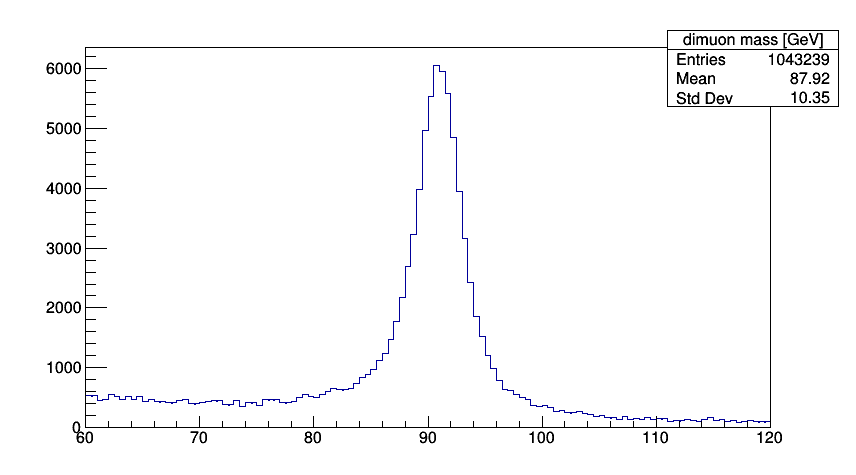
\includegraphics[width=0.48\linewidth]{c1.png}\hspace{-1 cm}}
\vspace{4 cm}
\end{frame}

\begin{frame}[fragile]{Taking this example apart (1/3)}
\vspace{0.25 cm}
\begin{itemize}
\item Femtocode always appears in quotes (like SQL). It is a big-data aggregation step in the midst of a traditional analysis.

\item A query is a ``workflow'' from source to aggregation, compiled and submitted as one unit.

e.g.\ {\tt\scriptsize source("dataset").define(X).define(Y).histogrammar(Z) }

\item Most Femtocode expressions are tiny (hence ``femto''), scattered throughout a Histogrammar aggregation:

\scriptsize
\begin{Verbatim}[commandchars=\\\{\}]
session.source(\textcolor{red}{"dataset"})
    .define(goodmuons = \textcolor{red}{"""..."""})  \textcolor{gray}{# define good muons}
    .filter(\textcolor{red}{"goodmuons.size >= 2"})  \textcolor{gray}{# cut on them}
    .define(dimuon = \textcolor{red}{"""..."""}      \textcolor{gray}{# define dimuons}
    .bundle(                        \textcolor{gray}{# plot their attributes}
        mass = bin(120, 0, 12, \textcolor{red}{"dimuon.mass"}),
        pt = bin(100, 0, 100, \textcolor{red}{"dimuon.pt"}),
        eta = bin(100, -5, 5, \textcolor{red}{"dimuon.eta"}),
        phi = bin(314, 0, 2*pi, \textcolor{red}{"dimuon.phi + pi"}),
                                    \textcolor{gray}{# also plot the muons}
        muons = explode(\textcolor{red}{"goodmuons"}, \textcolor{red}{"mu"}, bundle(
            pt = bin(100, 0, 100, \textcolor{red}{"mu.pt"}),
            eta = bin(100, -5, 5, \textcolor{red}{"mu.eta"}),
            phi = bin(314, -pi, pi, \textcolor{red}{"mu.phi"}))))
\end{Verbatim}
\end{itemize}
\end{frame}

\begin{frame}[fragile]{Taking this example apart (2/3)}
\begin{itemize}
\item Doubly nested loop by nesting functionals:

{\tt\small \textcolor{red}{muons.map(mu1 => muons.map(mu2 => f(mu1, mu2)))}}

is equivalent to

\small
\begin{minted}{python}
list_of_lists = []
for mu1 in muons:
    list_of_numbers = []
    for mu2 in muons:
        list_of_numbers.append(f(mu1, mu2))
    list_of_lists.append(list_of_numbers)
\end{minted}

\item There will someday be more convenient forms: \textcolor{red}{\tt pairs}, \textcolor{red}{\tt table}, \textcolor{red}{\tt filter}, \textcolor{red}{\tt flatten}, \textcolor{red}{\tt flatMap}, \textcolor{red}{\tt zip}, \textcolor{red}{\tt permutations}, etc.

\vspace{0.2 cm}
\textcolor{gray}{(This example would ideally use \textcolor{lightred}{\tt pairs}, to avoid double-counting, and \textcolor{lightred}{\tt flatten} to destructure the list-of-lists.)}
\end{itemize}
\end{frame}

\begin{frame}[fragile]{Taking this example apart (3/3)}
\vspace{0.2 cm}
\begin{itemize}
\item Type system requires domain of \textcolor{red}{\tt sqrt} to be guarded:

\scriptsize
\begin{Verbatim}[commandchars=\\\{\}]
  \textcolor{red}{sqrt(E**2 - px**2 - py**2 - pz**2)}

FemtocodeError: Function "sqrt" does not accept arguments with
the given types:

    sqrt(real)

    The sqrt function can only be used on non-negative numbers.

Check line:col 19:2 (pos 401):
      sqrt(E**2 - px**2 - py**2 - pz**2)
------^
\end{Verbatim}

\normalsize But this works:

\scriptsize
\begin{Verbatim}[commandchars=\\\{\}]
  \textcolor{red}{if E**2 - px**2 - py**2 - pz**2 >= 0:}
  \textcolor{red}{    sqrt(E**2 - px**2 - py**2 - pz**2)}
  \textcolor{red}{else:}
  \textcolor{red}{    None}
\end{Verbatim}

\normalsize

\item The compiler tracks each subexpression's interval of validity: \textcolor{red}{\tt\scriptsize E**2 - px**2 - py**2 - pz**2} is limited to \mbox{{\tt\scriptsize real(min=0, max=inf)}.\hspace{-1 cm}}

\vspace{0.2 cm}
In the future, we could use SymPy to discover \mbox{this algebraically.\hspace{-1 cm}}
\end{itemize}
\end{frame}

\begin{frame}{Another thing to notice}
\[
\begin{array}{ll}
\mbox{\textcolor{red}{\tt\scriptsize muons.map(mu1 => muons.map(\{mu2 =>}} & \\

\left.\renewcommand{\arraystretch}{0.7}\begin{array}{p{8 cm}}
\mbox{\textcolor{red}{\tt\scriptsize p1x = mu1.pt * cos(mu1.phi);}} \\
\mbox{\textcolor{red}{\tt\scriptsize p1y = mu1.pt * sin(mu1.phi);}} \\
\mbox{\textcolor{red}{\tt\scriptsize p1z = mu1.pt * sinh(mu1.eta);}} \\
\mbox{\textcolor{red}{\tt\scriptsize E1 = sqrt(p1x**2 + p1y**2 + p1z**2 + mumass**2);}}
\end{array}\right\} &
\mbox{only uses \textcolor{red}{\tt mu1}} \\
& \\
\left.\renewcommand{\arraystretch}{0.7}\begin{array}{p{8 cm}}
\mbox{\textcolor{red}{\tt\scriptsize p2x = mu2.pt * cos(mu2.phi);}} \\
\mbox{\textcolor{red}{\tt\scriptsize p2y = mu2.pt * sin(mu2.phi);}} \\
\mbox{\textcolor{red}{\tt\scriptsize p2z = mu2.pt * sinh(mu2.eta);}} \\
\mbox{\textcolor{red}{\tt\scriptsize E2 = sqrt(p2x**2 + p2y**2 + p2z**2 + mumass**2);}}
\end{array}\right\} &
\mbox{only uses \textcolor{red}{\tt mu2}} \\
& \\
\left.\renewcommand{\arraystretch}{0.7}\begin{array}{p{8 cm}}
\mbox{\textcolor{red}{\tt\scriptsize px = p1x + p2x;}} \\
\mbox{\textcolor{red}{\tt\scriptsize py = p1y + p2y;}} \\
\mbox{\textcolor{red}{\tt\scriptsize pz = p1z + p2z;}} \\
\mbox{\textcolor{red}{\tt\scriptsize E = E1 + E2;}} \\
\mbox{\textcolor{red}{\tt\scriptsize }} \\
\mbox{\textcolor{red}{\tt\scriptsize if E**2 - px**2 - py**2 - pz**2 >= 0:}} \\
\mbox{\textcolor{red}{\tt\scriptsize \hspace{0.25 cm}sqrt(E**2 - px**2 - py**2 - pz**2)}} \\
\mbox{\textcolor{red}{\tt\scriptsize else:}} \\
\mbox{\textcolor{red}{\tt\scriptsize \hspace{0.25 cm}None}}
\end{array}\right\} &
\mbox{uses both.} \\
\mbox{\textcolor{red}{\tt\scriptsize \}))}} & \\
\end{array}
\]
\end{frame}

\begin{frame}{Femtocode minimizes computation}
In most compilers, at least one of the two stanzas would be needlessly recomputed for every {\it pair} of muons. Physicists have learned to move these expressions out of the loop, possibly at the expense of readability.

\vfill
Femtocode's compiler turns every loop over objects into vectorized functions on individual fields. A by-product of this is that the functions depending on \textcolor{red}{\tt mu1} and \textcolor{red}{\tt mu2} decouple from the functions depending on \textcolor{red}{\tt (mu1, mu2)}.

\vfill
In fact, all duplicate expressions are computed exactly once. The {\it only} reason to use assignment is for clarity.
\end{frame}

\begin{frame}[fragile]{What the dimuon example expands to}
\begin{columns}[t]
\column{0.5\linewidth}
\tiny
\begin{Verbatim}[commandchars=\\\{\}]
Sized by muons[]@size:
    #0       := \textcolor{red}{cos}(muons[]-phi)
    #1       := \textcolor{red}{*}(muons[]-pt, #0)
    #2       := \textcolor{red}{**}(#1, \textcolor{darkgreen}{2})
    #3       := \textcolor{red}{sin}(muons[]-phi)
    #4       := \textcolor{red}{*}(muons[]-pt, #3)
    #5       := \textcolor{red}{**}(#4, \textcolor{darkgreen}{2})
    #6       := \textcolor{red}{sinh}(muons[]-eta)
    #7       := \textcolor{red}{*}(muons[]-pt, #6)
    #8       := \textcolor{red}{**}(#7, \textcolor{darkgreen}{2})
    #9       := \textcolor{red}{+}(#2, #5, #8, \textcolor{darkgreen}{0.011164})
    #10      := \textcolor{red}{sqrt}(#9)
\textcolor{gray}{type(#10) == real(0.105658, almost(inf))}

Sized by \#11@size:
    #11@size := \textcolor{red}{$explodesize}(muons[], muons[])
    #11      := \textcolor{red}{$explodedata}(#10, #11@size, (muons[]))
    #12      := \textcolor{red}{$explodedata}(#10, #11@size, (muons[], muons[]))
    #13      := \textcolor{red}{+}(#11, #12)
    #14      := \textcolor{red}{**}(#13, \textcolor{darkgreen}{2})
    #15      := \textcolor{red}{$explodedata}(#1, #11@size, (muons[]))
    #16      := \textcolor{red}{$explodedata}(#1, #11@size, (muons[], muons[]))
    #17      := \textcolor{red}{+}(#15, #16)
    #18      := \textcolor{red}{**}(#17, \textcolor{darkgreen}{2})
    #19      := \textcolor{red}{-}(#14, #18)
    #20      := \textcolor{red}{$explodedata}(#4, #11@size, (muons[]))
    #21      := \textcolor{red}{$explodedata}(#4, #11@size, (muons[], muons[]))
    #22      := \textcolor{red}{+}(#20, #21)
    #23      := \textcolor{red}{**}(#22, \textcolor{darkgreen}{2})
    #24      := \textcolor{red}{-}(#19, #23)
    #25      := \textcolor{red}{$explodedata}(#7, #11@size, (muons[]))
    #26      := \textcolor{red}{$explodedata}(#7, #11@size, (muons[], muons[]))
\end{Verbatim}

\column{0.5\linewidth}
\tiny
\begin{Verbatim}[commandchars=\\\{\}]

    #27      := \textcolor{red}{+}(#25, #26)
    #28      := \textcolor{red}{**}(#27, \textcolor{darkgreen}{2})
    #29      := \textcolor{red}{-}(#24, #28)
    #30      := \textcolor{red}{>=}(#29, \textcolor{darkgreen}{0})
    #31      := \textcolor{red}{<}(#29, \textcolor{darkgreen}{0})
    #32      := \textcolor{red}{-}(#24, #28)
    #33      := \textcolor{red}{sqrt}(#32)
    #34      := \textcolor{red}{if}(#30, #31, #33, \textcolor{darkgreen}{None})
\textcolor{gray}{type(#34) == union(null, real(0, almost(inf)))}
\end{Verbatim}

\vspace{0.3 cm}
\hfill \fbox{\begin{minipage}{2.6 cm}
\scriptsize\raggedright {\tt muons[]-pt}, {\tt muons[]-phi}, {\tt muons[]-eta}, {\tt muons[]@size}, and everything that starts with a {\tt \#} is (at least conceptually) a big array of values.

\vspace{0.2 cm}
All functions except \textcolor{red}{\tt \$explode*} are ideally suited to GPU acceleration.
\end{minipage}}
\end{columns}
\end{frame}

\begin{frame}[fragile]{Execution engine: objects become arrays}
\vspace{0.3 cm}
\textcolor{darkblue}{\normalsize Muon object schema:}

\scriptsize
\begin{Verbatim}[commandchars=\\\{\}]
\textcolor{darkgreen}{muons} = \textcolor{blue}{collection}(\textcolor{blue}{record}(
            \textcolor{darkgreen}{pt} = \textcolor{blue}{real}(0, almost(inf)),
            \textcolor{darkgreen}{eta} = \textcolor{blue}{real},
            \textcolor{darkgreen}{phi} = \textcolor{blue}{real}(-pi, pi)))
\end{Verbatim}

\vspace{0.3 cm}
\textcolor{darkblue}{\normalsize Physical representation:}

\scriptsize
\begin{minted}{python}
data = {
    "muons[]-pt":   [31.0960, 9.7620, 8.1769, ...,
                       5.2730, 4.7240, 8.5879],    # (length 132274)
    "muons[]-phi":  [-0.4814, -0.1242, -0.1185, ...,
                       1.2469, -0.2067, -1.7541],  # (length 132274)
    "muons[]-eta":  [0.8816, 0.9243, 0.9226, ...,
                       -0.9911, 0.9532, -0.2635],  # (length 132274)
    "muons[]@size": [7, 1, 4, ..., 4, 0, 1]}       # (length 48131)
\end{minted}

\vspace{0.3 cm}
\textcolor{darkblue}{\normalsize Dimuon run produces:}

\scriptsize
\begin{Verbatim}[commandchars=\\\{\}]
\textcolor{darkgreen}{masses} = \textcolor{blue}{collection}(\textcolor{blue}{collection}(\textcolor{blue}{union}(\textcolor{blue}{null}, \textcolor{blue}{real}(0, almost(inf)))))
\end{Verbatim}

\scriptsize
\begin{minted}{python}
output = {
    "#34":          [0.2113, 6.2386, 5.7978, ...,
                       13.1108, 0.2113, 0.2113],   # (length 584642)
    "#11@size":     [7, 7, 7, ..., 0, 1, 1]}       # (length 180405)
\end{minted}
\end{frame}

\end{document}
